\section{Motivation}

In order to ensure the ground handling employees work at their optimal performance, regarding both attention(safety) and speed, their individual motivation must be accounted for. Studies on this subject argues that; "intrinsic motivation (based in interest) and autonomous extrinsic motivation (based in importance) are both related to performance, satisfaction, trust, and well-being in the workplace" \cite{GAGNE}.

It is important to maintain autonomous intrinsic motivation so that an employee's level of specific competence matches the requirements for that specific task; the task must not be too difficult or too simple. Failing to meet this will result in amotivation towards certain tasks, because the employee feels it is not what is important, or that they are incompetent. Although tasks will occur in a ground handling environment, an extrinsic motivation can promote autonomous behaviour to get a raise or so the boss won't become upset. All of the factors shown in \ref{Movation}.

\begin{figure}
\centering
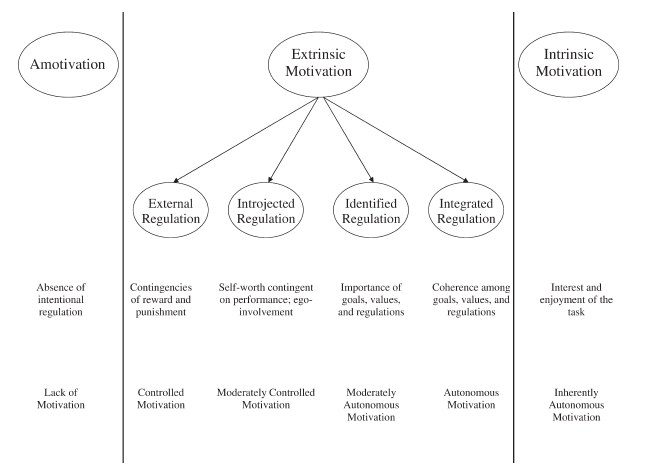
\includegraphics[width=\textwidth]{Grafik/Motivation}
\caption{Different types of motivation}
\label{Movation}
\end{figure}

A model of job characteristic introduced by Hackman and Oldham, which suggested the most effective factors of building motivation is through optimal job design \cite{HACKMAN}, as shown in \ref{Hackman}.

\begin{figure}
\centering
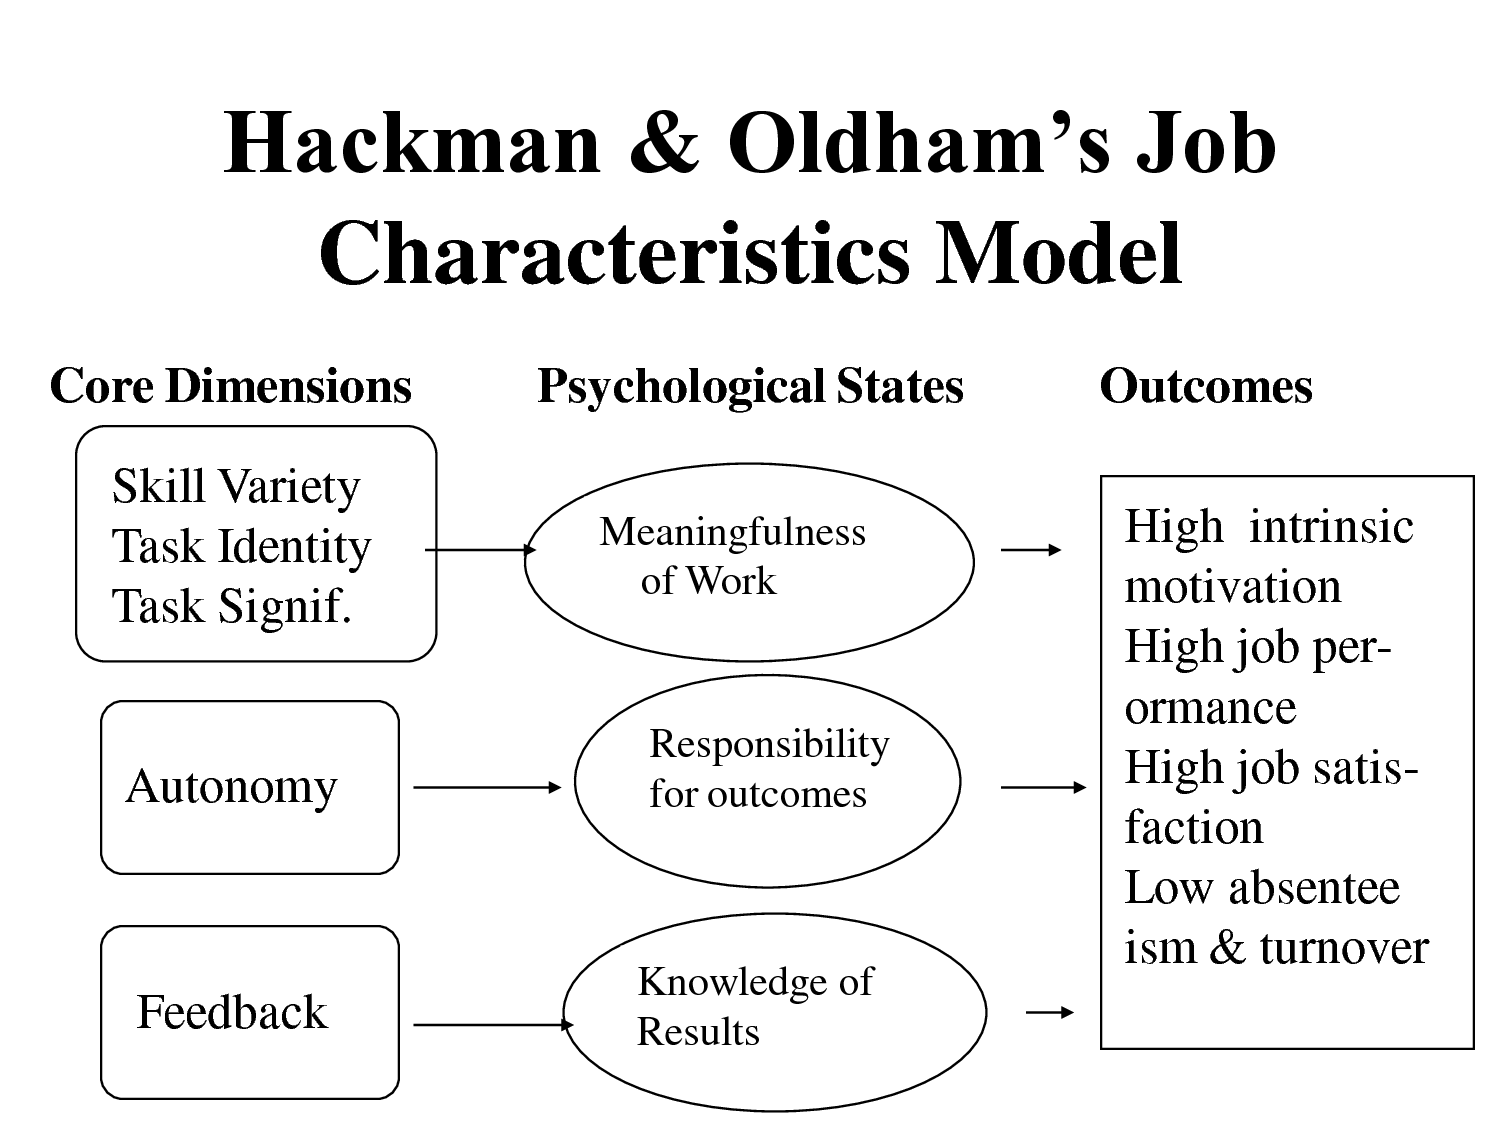
\includegraphics[width=\textwidth]{Grafik/Hackman}
\caption{Model of job characteristic \cite{HACKMAN}}
\label{Hackman}
\end{figure}

\begin{itemize}
\item provide variety, involve completion of a whole, and have a positive impact on the lives of others;
\item afford considerable freedom and discretion to the employee
\item provide meaningful performance feedback.
\end{itemize}

Constructive feedback can influence autonomous motivation, but it also suggests that the supervisors and managers are important in creating a work environment, consisting of a mix of intrinsic motivation and extrinsic motivation, which is superior in situations that include both complex tasks that are interesting and less complex tasks that require discipline. 
